\subsection{Customer Choice Dynamics}
We first show that every customer exhibits the following behavior: until (s)he reaches the phase transition point $i_0(t)$, she visits $A$ only due to the exogeneity paramaeter, and after that (s)he always visits merchant $A$ till she receives the reward.
This behavior is cyclic, and repeats after the first reward redemption.

\begin{lemma} $V(i)$ is an increasing function in $i$ if the following condition holds:
\begin{equation}
R > \frac{(1-\lambda)v}{1-\beta}
\end{equation}
And further, $V(i)$ can be evaluated as:
\begin{equation}
V(i) = \max\left\{ \frac{\lambda \beta V(i+1)+(1-\lambda)v}{1-(1-\lambda)\beta}, \beta V(i+1) \right\}
\end{equation}
\end{lemma}

\begin{proof}
First we show that $V(i)$ is an increasing function in $i$ by induction. We first show that if the condition above is satisfied, $V(k-1) < V(k) = R$. Suppose not, so $V(i) \geq R$. Then we have:
\begin{align*}
V(k-1) &= \lambda \beta V(k) + (1-\lambda)(v+\beta V(k-1)) \\
&= \frac{\lambda \beta R + (1-\lambda)v}{1-(1-\lambda)\beta} \\
&< \frac{\lambda \beta R + (1-\beta)R}{1-(1-\lambda)\beta} \\
&= \frac{R(1-(1-\lambda)\beta)}{1-(1-\lambda)\beta} = R
\end{align*}
But this is a contradiction, so $V(k-1) < V(k)$. Now assume $V(i+1) < V(i+2)$ for some $i < k-2$, we will show that this implies $V(i) < V(i+1)$. Suppose not, so $V(i) \geq V(i+1)$. As we did before we may upper bound $V(i)$.
\begin{align*}
V(i) &= \lambda \beta V(i+1) + (1-\lambda)(v+\beta V(i)) \\
&\leq (1-\lambda)v + \beta V(i) \\
\iff V(i) &\leq \frac{(1-\lambda)v}{1-\beta}
\end{align*}
But because $V(i+1) < V(i+2)$, we may lower bound $V(i+1)$.
\begin{align*}
V(i+1) &\geq \lambda \beta V(i+2) + (1-\lambda)(v+\beta V(i+1)) \\
&= (1-\lambda)v + (1-\lambda)\beta V(i+1) + \lambda \beta V(i+2) \\
&> (1-\lambda)+\beta V(i+1) \\
\iff V(i+1) &> \frac{(1-\lambda)v}{1-\beta}
\end{align*}
Again, we have a contradiction, so $V(i) < V(i+1)$, and $V(i)$ is an increasing function in $i$. Now we prove the second claim. We have the following:
\begin{align*}
V(i) &= \lambda \beta V(i+1) + (1-\lambda)\max\{v +\beta V(i), \beta V(i+1) \} \\
&= \max\{\lambda \beta V(i+1) + (1-\lambda)(v+\beta V(i)), \beta V(i+1) \}
\end{align*}

Assuming $V(i)$ is the left term in the above maximum, we may solve the equation for that term.
\begin{gather*}
V(i) = \lambda \beta V(i+1) + (1-\lambda)(v+\beta V(i)) \\
(1-(1-\lambda)\beta) V(i) = \lambda \beta V(i+1) + (1-\lambda)v \\
V(i) = \frac{\lambda \beta V(i+1) + (1-\lambda)v}{1-(1-\lambda)\beta}
\end{gather*}
And we get our claim.
\end{proof}

\begin{theorem} Assuming $V(i)$ is an increasing function in $i$, a phase transition occurs after the consumer makes $i_0$ visits to firm $A$, which evaluates to:
\begin{align*}
i_0 &= k - \left\lfloor \log_{\beta}\left(\frac{v}{R(1-\beta)}\right)\right\rfloor \\
&\equiv k-\Delta
\end{align*}
\end{theorem}

\begin{proof}
First we solve for the condition on $V(i+1)$ for us to choose firm $A$ over $B$ willingly.
\begin{gather*}
\beta V(i+1) > \frac{\lambda \beta V(i+1) + (1-\lambda)v}{1-(1-\lambda)\beta} \\
\iff \beta V(i+1) \left(1-\frac{\lambda}{1-(1-\lambda)\beta} \right) > \left(\frac{1-\lambda}{1-(1-\lambda)\beta} \right) v \\
\iff \beta V(i+1) \left(\frac{1-(1-\lambda)\beta -\lambda}{1-(1-\lambda)\beta} \right) > \left(\frac{1-\lambda}{1-(1-\lambda)\beta} \right) v \\
\iff \beta V(i+1) \left(\frac{(1-\lambda)(1-\beta)}{1-(1-\lambda)\beta} \right) > \left(\frac{1-\lambda}{1-(1-\lambda)\beta} \right) v \\
\iff \beta V(i+1) > \frac{v}{1-\beta} \\
\iff V(i+1) > \frac{v}{\beta(1-\beta)}
\end{gather*}
Let $i_0$ be the minimum state $i$ such that the above holds, so in particular $V(i_0) \le \frac{v}{\beta(1-\beta)}$ but $V(i_0+1) > \frac{v}{\beta(1-\beta)}$. We know because $V$ is increasing in $i$ (still need to prove), this point is indeed a phase transition: $V(i) > \frac{v}{\beta(1-\beta)}$ for all $i > i_0$, so after this point, the customer always chooses firm $A$. We may compute $V(i_0)$ easily using this fact.
\begin{equation*}
V(i_0) = \beta V(i_0+1) = \cdots = \beta^{k-i_0}V(k) = \beta^{k-i_0}R
\end{equation*}
Thus, we have the following:
\begin{gather*}
\beta^{k-i_0} \le \frac{v}{R\beta(1-\beta)} < \beta^{k-(i_0+1)} \\ 
\iff k-i_0 \ge \log_{\beta}\left(\frac{v}{R\beta(1-\beta)} \right) > k-(i_0+1) \\
\iff i_0 \le k - \log_{\beta}\left(\frac{v}{R(1-\beta)} \right) + 1 < i_0 + 1\\
\iff i_0 = k - \left\lfloor \log_{\beta}\left(\frac{v}{R(1-\beta)}\right) \right\rfloor \equiv k-\Delta
\end{gather*}
\end{proof}

Now we assume the look-ahead factor of a customer is drawn from some distribution $t \sim T$. The phase transition of the customer's DP will now depend on $t$.
\begin{equation*}
  i_0(t)=\begin{cases}
    i_0, & \text{if $t \geq \Delta$}.\\
    k-t, & \text{otherwise}.
  \end{cases}
\end{equation*}

In this section, we focus on a very simple threshold distribution given by the following.
\begin{equation*}
  t=\begin{cases}
    t_1\geq \Delta, & \text{wp } p,\\
    0, & \text{wp } 1-p.
  \end{cases}
\end{equation*}

\subsection{Merchant Objective Dynamics}
\subsubsection{Non Strategic Merchant $B$, and Equal Promotion Budgeting}
First we look into the case when merchant $B$ does not strategize over its discount value $v$, and when merchant $A$ sets its reward parameters so as to have equal budgets for promosionts as $B$: \ie~ $R = k v$.
\begin{theorem}
Given $\lambda~\sim Unif(0,b)$, merchant $A$ sets its reward parameter $k = \frac{e}{1-\beta}$ at small values of $b$ and $k = \frac{e^{(1-\beta)t_1}}{1-\beta}$ for larger values.
\end{theorem}
\begin{proof}
First merchant $A$'s objective evaluates to the following:
\begin{align*}
\underset{k}\max\{RoR_A\} \Leftrightarrow & \underset{k}\max\left\{\underset{\lambda}E\left[\frac{\lambda k}{k-\Delta(1-\lambda)}\right]\right\}\\
                          \Leftrightarrow & \underset{k}\max\left\{ \frac{1}{b}\int_{0}^{b} \frac{\lambda k}{k-\Delta(1-\lambda)}d\lambda \right\}\\
                          \Leftrightarrow & \underset{k}\max\left\{ \frac{k}{\Delta^2 b}\left(\Delta b - (k-\Delta)\log\left(\frac{k-\Delta(1-b)}{k-\Delta}\right)\right) \right\}\\
                          \Leftrightarrow & \underset{k} \max\left\{\frac{k}{\Delta}\left(1-\frac{k-\Delta}{b\Delta}\log\left(\frac{k-\Delta(1-b)}{k-\Delta}\right)\right)\right\}
\end{align*}
Now let $\theta = \frac{\Delta}{k}$. Then maximizing the above function is equivalent to maximizing the following function w.r.t. $\theta$ with keeping in mind the range that $\theta$ can follow.
\beq
\underset{k}\max\{RoR_A\} \Leftrightarrow \underset{\theta}\max\{f(\theta)\} \Leftrightarrow \underset{\theta}\max\left\{ \frac{1}{\theta} \left(1-\frac{1-\theta}{b\theta}\log\left(1 + \frac{b\theta}{1-\theta}\right)\right)\right\} 
\eeq
Let's look at the quantity $\frac{\Delta}{k}$.
\begin{align*}
\frac{\Delta}{k} = \frac{\log_\beta\left(\frac{1}{k(1-\beta)}\right)}{k} \sim \frac{\log(k(1-\beta))}{k(1-\beta)} 
\end{align*}
Now this value is maximized at $k = \frac{e}{1-\beta}$ and minimized at the maximum possible value of $k$ which is bounded above by $\frac{e^{(1-\beta)t_1}}{1-\beta}$ from the assumption of $t_1 \ge \Delta$.

When $b$ is small, the function $f(\theta)$ can be approximated by taking the second degree terms for the term inside the log. This gives:

\begin{align*}
f(\theta) \sim & \frac{1}{\theta} \left(1-\frac{1-\theta}{b\theta}\left(\frac{b\theta}{1-\theta} - \frac{\left(\frac{b\theta}{1-\theta}\right)^2}{2}\right)\right)\\
          = & \frac{b}{2(1-\theta)}
\end{align*}
Clearly $f(\theta)$ is maximized when $\theta$ is maximized. This happens as shown above at $k = \frac{e}{1-\beta}$

Whereas when $b$ is large, $f'(\theta)$ can be shown to be negative. Hence we get our result.

\end{proof}

Note that under equal-budgeting, we need $k > \frac{1-\lambda}{1-\beta}$ for $V$ to be increasing. We meet this condition when $k = \frac{e}{1-\beta} > \frac{1}{1-\beta} \geq \frac{1-\lambda}{1-\beta}$. Figure~\ref{fig:phase_trans} shows the percentage of visits needed for a ``forward-looking'' consumer to adopt the reward program as a function of $\beta$. (Here we should add our comments on cash back computations).

\begin{figure}[h!]
\begin{centering}
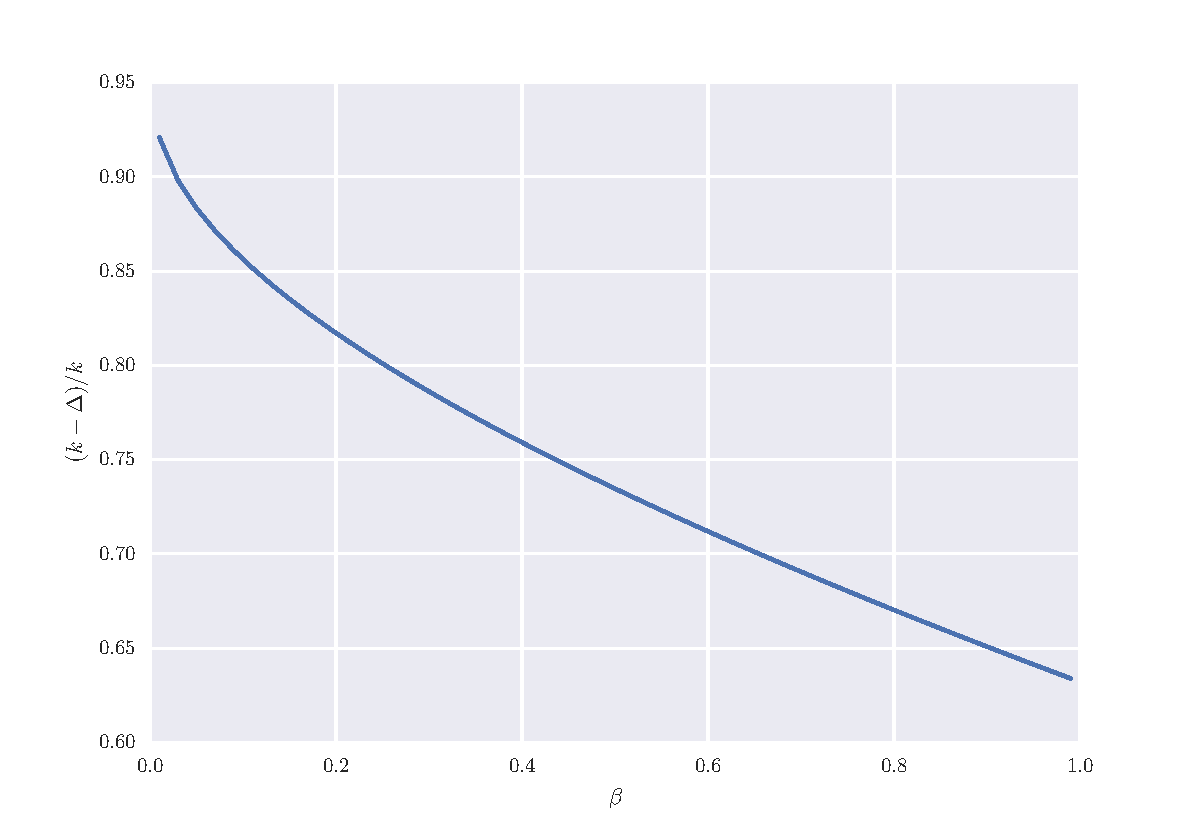
\includegraphics[scale = 0.75]{./figures/phase_trans.pdf}
\caption{We assume $k = e/(1-\beta)$ and equal-budgeting. The plot shows the percentage of extraneous visits needed for a ``forward-looking'' consumer needed to adopt the reward program as a function of $\beta$.}
\label{fig:phase_trans}
\end{centering}
\end{figure}

Now we consider the expected revenues of each firm under these conditions.

\beq
\underset{\lambda, t}E[RoR_A] = pk(1-v)\frac{1}{b}\int_0^b \frac{\lambda}{k-(1-\lambda)\Delta} \mbox{ } d\lambda + (1-p)(1-v)\frac{b}{2}
\eeq

\beq
\underset{\lambda, t}E[RoR_B] = pk(1-v)\frac{1}{b}\int_0^b \frac{1-\lambda}{k-(1-\lambda)\Delta} \mbox{ } d\lambda + (1-p)(1-v)\left(1-\frac{b}{2}\right)
\eeq

First notice that the ratio of expected revenues is independent of $v$, the price difference of the two firms. We observe this behavior in our simulations as well. Figure~\ref{fig:eq_budg_vary_v} shows the revenue rates of $A$ and $B$ as a function of $b$ for different values of $v$. We see that the relative rates do not vary with $v$; changing $v$ only changes the absolute revenue rates of each firm, putting more money into the rewards given out. We see that $b$ must be pretty large for firm $A$ to make more money than firm $B$. 

\begin{figure}[h!]
\begin{centering}
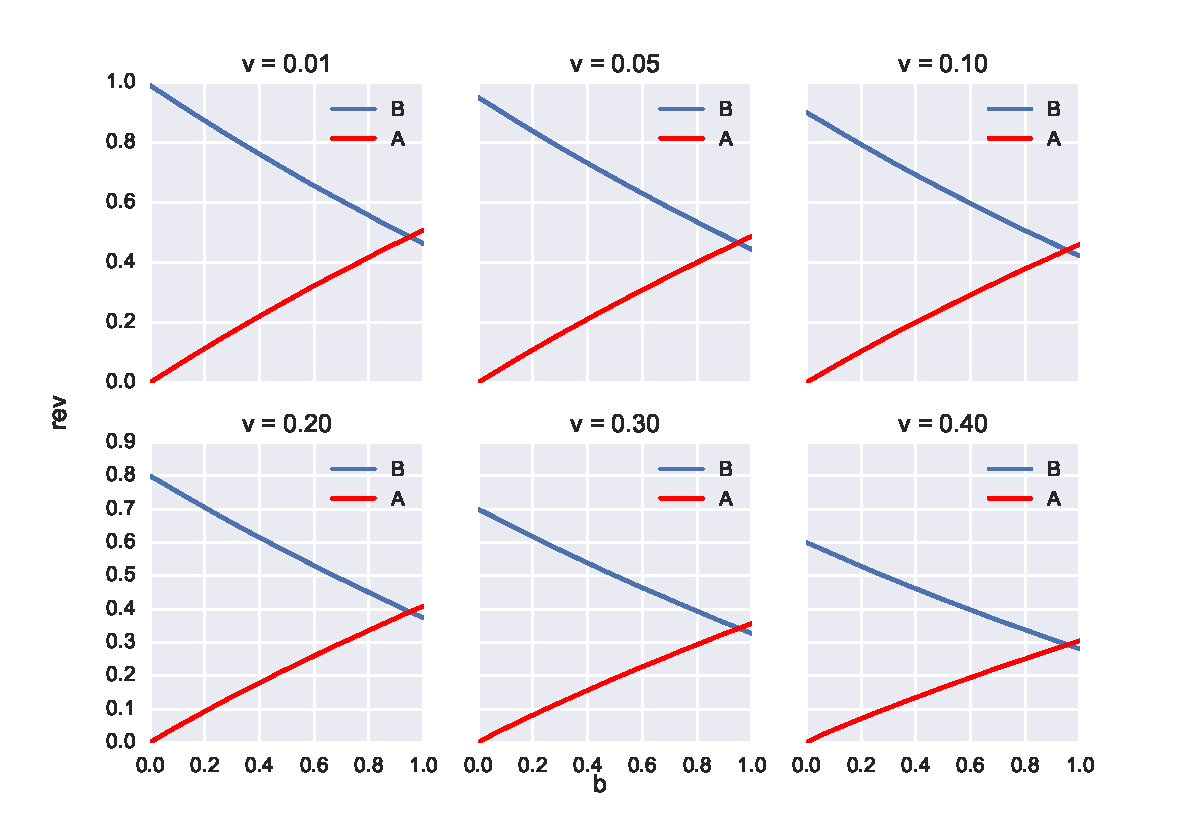
\includegraphics[scale = 0.75]{./figures/eq_budg_vary_v_p05.pdf}
\caption{Rates of revenue for $A$ and $B$ with equal-budgeting as a function of $b$ for various $v$. Fixed $p = 0.5$, $\beta = 0.9$ and $k = e/(1-\beta)$.}
\label{fig:eq_budg_vary_v}
\end{centering}
\end{figure}

[Not sure if we should include] We may solve for the $b$ such that the expected revenues are equal, which occurs if when the following holds (excluding work for now).
\begin{equation*}
b-\frac{2k(k-\Delta)p}{(1-p)b\Delta^2}\log \left(\frac{k-(1-b)\Delta}{k-\Delta} \right) = 1-\frac{p}{1-p} \frac{2k-\Delta}{\Delta}
\end{equation*}

Note from the above that $p$, the probability of a consumer being ``forward-looking'' does affect the ratio of expected rates of revenue. Figure~\ref{fig:eq_budg_vary_p} shows simulation results for the rates of revenue of $A$ and $B$ for various values of $p$ with everything else fixed. We see that as $p$ increases, the $b$ required for the reward program to become more profitable than not using one decreases.

\begin{figure}[h!]
\begin{centering}
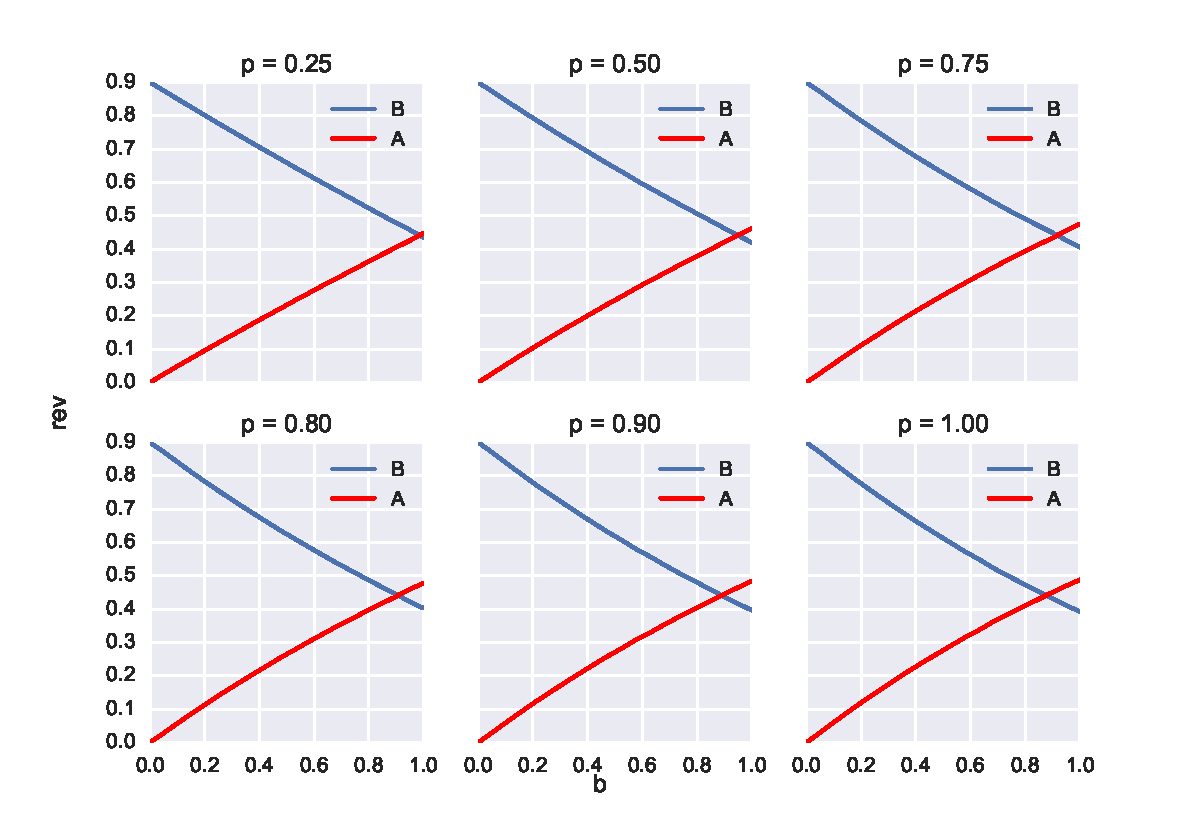
\includegraphics[scale = 0.75]{./figures/eq_budg_vary_p_v01.pdf}
\caption{Rates of revenue for $A$ and $B$ with equal-budgeting as a function of $b$ for various $p$. Fixed $v = 0.1$, $\beta = 0.9$ and $k = e/(1-\beta)$.}
\label{fig:eq_budg_vary_p}
\end{centering}
\end{figure}

\subsubsection{Non Strategic Merchant $B$, and Unequal Promotion Budgeting}

Now we consider scenarios in which firms $A$ and $B$ have different budgets. First we consider the case where the budgets are still proportional, i.e. $R = \alpha \cdot kv$ for some fixed $\alpha$. Now the expected rate of revenue of $A$ is given by the following, while that of firm $B$ is unchanged. Therefore the ratio of expected revenue rates may now depend on $v$.
\beq
\underset{\lambda, t}E[RoR_A] = pk(1-\alpha v)\frac{1}{b}\int_0^b \frac{\lambda}{k-(1-\lambda)\Delta} \mbox{ } d\lambda + (1-p)(1-\alpha v)\frac{b}{2}
\eeq

Following the same logic of Theorem 3.2, the expected revenue rate of $A$ is maximized at $k = \frac{e}{\alpha(1-\beta)}$ at small values of $b$ (need to do again for larger values).

\begin{lemma}
The objective function for the above look-ahead distribution is given by:
\begin{equation*}
f(k) = \frac{\lambda (k-R)p}{k-(1-\lambda)\Delta}+\frac{\lambda (k-R)(1-p)}{k-(1-\lambda)t_0}
\end{equation*}
\end{lemma}

\begin{proof}
\begin{align*}
E_t\left(\frac{k-R}{\frac{i_0(t)}{\lambda}+k-i_0(t)} \right) &= \frac{(k-R)p}{\frac{i_0}{\lambda}+k-i_0}+\frac{(k-R)(1-p)}{\frac{k-t_0}{\lambda}+k-(k-t-0)} \\
&= \frac{\lambda(k-R)p}{i_0+\lambda(k-i_0)}+\frac{\lambda(k-R)(1-p)}{k-t_0+t_0\lambda} \\
&= \frac{\lambda(k-R)p}{k-\Delta+\lambda(\Delta)}+\frac{\lambda(k-R)(1-p)}{k-t_0+t_0\lambda} \\
&= \frac{\lambda (k-R)p}{k-(1-\lambda)\Delta}+\frac{\lambda (k-R)(1-p)}{k-(1-\lambda)t_0} \equiv f(k)
\end{align*}
\end{proof}

We wish to maximize this objective function for $k>\Delta$ (otherwise $i_0$ would be negative). Next, we will characterize the conditions under which we can maximize the function and what the maxima are.

\begin{lemma}
If $(1-\lambda)t_0 \leq R \leq (1-\lambda)\Delta$, the above objective function has real-valued critical points.
\end{lemma}

\begin{proof}
First we differentiate $f(k)$.
\begin{align*}
\frac{df}{dk} &= \frac{\lambda(k-(1-\lambda)\Delta)-\lambda(k-R)p}{(k-(1-\lambda)\Delta)^2}+\frac{\lambda(1-p)(k-(1-\lambda)t_0)-\lambda(k-R)(1-p)}{(k-(1-\lambda)t_0)^2} \\
&= \frac{\lambda p(R-(1-\lambda)\Delta)}{(k-(1-\lambda)\Delta)^2} + \frac{\lambda(1-p)(R-(1-\lambda)t_0)}{(k-(1-\lambda)t_0)^2}
\end{align*}
Setting equal to zero and solving for $k$ we get the following. Let $c_1 = R-(1-\lambda)\Delta$ and $c_2 = R-(1-\lambda)t_0$.
\begin{gather*}
pc_1(k-(1-\lambda)t_0)^2 = -(1-p)c_2(k-(1-\lambda)R)^2 \\
\iff (pc_1)k^2-(2pc_1(1-\lambda))k+(pc_1(1-\lambda)^2t_0^2 = (-(1-p)c_2)k^2+(2(1-p)(1-\lambda)c_2\Delta)k-((1-p)c_2(1-\lambda)^2\Delta^2) \\
\iff (pc_1+(1-p)c_2)k^2-2(1-\lambda)(pc_1t_0+(1-p)c_2\Delta)k+(1-\lambda)^2(pc_1t_0^2+(1-p)c_2\Delta^2) = 0
\end{gather*}
For the above to have real-valued solutions, we need:
\begin{gather*}
4(1-\lambda)^2(pc_1t_0+(1-p)c_2\Delta)^2 - 4(pc_1+(1-p)c_2)(1-\lambda)^2(pc_1t_0^2+(1-p)c_2\Delta^2) \geq 0 \\
\iff p^2c_1^2t_0^2+(1-p)^2c_2^2\Delta^2+2p(1-p)c_1c_2t_0\Delta - p^2c_1^2t_0^2+(1-p)^2c_2^2\Delta^2+p(1-p)c_1c_2t_0^2+p(1-p)c_1c_2\Delta^2 \geq 0 \\
\iff p(1-p)c_1c_2(2t_0\Delta-\Delta^2-t_0^2) \geq 0 \\
\iff -p(1-p)c_1c_2(t_0-\Delta)^2 \geq 0 \\
\iff -p(1-p)c_1c_2 \geq 0 \\
\iff c_1c_2 \leq 0
\end{gather*}
The constraint that $c_1c_2 \leq 0$ means $(R-(1-\lambda)\Delta)(R-(1-\lambda)t_0) \leq 0$. Because $R \geq 0$, $(1-\lambda) \geq 0$ and $t_0 < \Delta$, we also have that $(R-(1-\lambda)\Delta) < (R-(1-\lambda)t_0)$. So we must have:
\begin{gather*}
(R-(1-\lambda)\Delta) \leq 0 \leq (R-(1-\lambda)t_0) \\
\iff (1-\lambda)t_0 \leq R \leq (1-\lambda)\Delta
\end{gather*}
\end{proof}

Note that $\Delta$ depends on $R$, so the above inequality is more complicated than as written. TODO - see if we can get a nice inequality for $R$ not in terms of $\Delta$. (Can also add a sample plot here). \\

Now need to check that this is actually a maximum.

\section{When should a store offer a reward?}

Notice the revenue rate function $f(k)$, fixing $\beta$, $t_0$, $p$, $R$ and $\lambda$, approaches $\lambda$ as $k \rightarrow \infty$. This limit makes sense, as $k$ approaching $\infty$ means that no reward will be given, so all visits to $B$ will be exogenous, with a revenue rate of $\lambda$. One question that we may find interesting is when it is impossible to beat the revenue rate of $\lambda$ (supposing $R$ is fixed) and thus not offer a reward at all. Even if fixing $R$ is not very realistic, understanding the objective function as a function of $\lambda$ may give us insight into what to set $R$. \\

Let's fix $\beta$, $p$, $R$ and let $t_0 = 0$ for now (for simplicity - can go in later and add more general case next). We wish to find the set of $\lambda \in [0,1]$ such that $f(k) \leq \lambda$ on $k \geq \Delta$: the $\lambda$'s for which we can not beat revenue rate of $\lambda$. I believe that there will always be some $\lambda_0$ such that for all $\lambda < \lambda_0$, we can increase the revenue rate by offering a reward and for all $\lambda \geq \lambda_0$, we cannot increase the revenue rate by offering a reward. (Note: I have not finished with the full proof of this yet, but going to write-up some ideas so far). \\

\begin{lemma} Fix $R > 0$, $\beta$, $p$, $v$ and $t_0 = 0$. Then $f(\Delta) \leq \lambda$ if and only if $\lambda \geq \frac{p(\Delta-R)}{\Delta-(\Delta-R)(1-p)}$. Note that when equality holds in the second inequality, it does in the first as well. \end{lemma}
\begin{proof}
We have:
\begin{align*}
f(\Delta) &= \frac{\lambda p (\Delta-R)}{\Delta-(1-\lambda)\Delta}+\frac{\lambda (1-p)(\Delta-R)}{\Delta} \\
&= \frac{p(\Delta-R)}{\Delta}+\frac{\lambda(1-p)(\Delta-R)}{\Delta} \\
&= \frac{(\Delta-R)(\lambda(1-p)+p)}{\Delta}
\end{align*}
Then:
\begin{gather*}
\frac{(\Delta-R)(\lambda(1-p)+p)}{\Delta} \leq \lambda \\
\iff \lambda-\frac{(\Delta-R)\lambda(1-p)}{\Delta} \geq \frac{p(\Delta-R)}{\Delta} \\
\iff \lambda \left(\frac{\Delta-(\Delta-R)(1-p)}{\Delta}\right) \geq \frac{p(\Delta-R)}{\Delta} \\
\iff \lambda \geq \frac{p(\Delta-R)}{\Delta-(\Delta-R)(1-p)}
\end{gather*}
Note for the last step above, we need $\Delta-(\Delta-R)(1-p) > 0$. But because $\Delta, R, (1-p) \geq 0$ then if $(\Delta-R) \leq 0$, the condition will always be satisfied (if $(\Delta-R) = 0$, $\Delta = R > 0$ and value is positive). And if $(\Delta-R) > 0$, $(1-p)(\Delta-R) \leq (\Delta-R) < \Delta$, so $\Delta-(\Delta-R)(1-p) > 0$.
\end{proof}

I believe the above threshold $\frac{p(\Delta-R)}{\Delta-(\Delta-R)(1-p)}$ is our desired $\lambda_0$. To show this we need to show that $f(\Delta)$ is a necessary and sufficient condition for $f(k)$ not exceeding $\lambda$ on $k \geq \Delta$. Clearly it is a necessary condition, so we just need to show it is sufficient. I believe the best way to do this is to show that for these $\lambda$, no critical points that are maxima exist in the range $[\Delta, \infty)$. If this is the case, then the max will occur at the the endpoints, which we have already argued will not be greater than $\lambda$. First we prove some lemmas about the roots of $f'$, assuming they are real-valued. \\

\begin{lemma}
If $p(R-(1-\lambda)\Delta)+(1-p)R > 0$, the objective function $f(k)$ (when $t_0 = 0$) has at least one real-valued critical point with value at least $(1-\lambda)\Delta$.
\end{lemma}
\begin{proof}
First note that we need $R-(1-\lambda)\Delta \leq 0 \leq R-(1-\lambda)t_0 = R$ for $f'$ to have real roots. The roots of $f'$ are given by:
\begin{equation*}
x = \frac{(1-\lambda)((1-p)R\Delta) \pm (1-\lambda)\Delta(-p(1-p)(R-(1-\lambda)\Delta)R)^{\frac{1}{2}}}{p(R-(1-\lambda)\Delta)+(1-p)R} \equiv C\pm D
\end{equation*}
We will show that $C = 
\frac{(1-\lambda)((1-p)R\Delta)}{p(R-(1-\lambda)\Delta)+(1-p)R} \geq (1-\lambda) \Delta$. Then $f'$ has at most one root less than $(1-\lambda)\Delta$; because if $C \geq (1-\lambda)\Delta$, for every $D$ it is not possible for both $C+D$ and $C-D$ to be less than $(1-\lambda)\Delta$. Note that $(1-\lambda)(1-p)R\Delta \geq 0$ and $p(R-(1-\lambda)\Delta) \leq 0$ and by assumption, the denominator of $C$ is positive as well. Therefore, we have:
\begin{align*}
C &= \frac{(1-\lambda)(1-p)R\Delta}{p(R-(1-\lambda)\Delta)+(1-p)R} \\
&\geq \frac{(1-\lambda)(1-p)R\Delta}{(1-p)R} = (1-\lambda)\Delta
\end{align*}
because $(1-p)R \geq (1-p)R+p(R-(1-\lambda)\Delta) > 0$.
\end{proof}

Note that the above lemma applies to any choice of parameters as long as that denominator is positive. Hopefully we can use it to understand the objective function in more general settings as well.

\begin{lemma} If $\lambda \geq \frac{p(\Delta-R)}{\Delta-(\Delta-R)(1-p)}$, the objective function $f(k)$ (when $t_0 = 0$) has at most one real-valued critical point greater than $\Delta$. \end{lemma}
\begin{proof}
Again note that we need $R-(1-\lambda)\Delta \leq 0 \leq R-(1-\lambda)t_0 = R$ for $f'$ to have real roots. The roots of $f'$ are given by:
\begin{equation*}
x = \frac{(1-\lambda)((1-p)R\Delta) \pm (1-\lambda)\Delta(-p(1-p)(R-(1-\lambda)\Delta)R)^{\frac{1}{2}}}{p(R-(1-\lambda)\Delta)+(1-p)R} \equiv C\pm D
\end{equation*}
We will show that $C = 
\frac{(1-\lambda)((1-p)R\Delta)}{p(R-(1-\lambda)\Delta)+(1-p)R} \leq \Delta$. Then $f'$ has at most one root great than $\Delta$; because if $C \leq \Delta$, for every $D$ it is not possible for both $C+D$ and $C-D$ to be greater than $\Delta$. Note that $(1-\lambda)(1-p)R\Delta \geq 0$ and $p(R-(1-\lambda)\Delta) \leq 0$. If $p(R-(1-\lambda)\Delta)+(1-p)R < 0$, then $C < 0 \leq \Delta$ and we are done. So we focus on the case that $p(R-(1-\lambda)\Delta)+(1-p)R > 0$. \\

We will think of $C$ as a function of $\lambda$.First we show that for $\lambda' = \frac{p(\Delta-R)}{\Delta-(\Delta-R)(1-p)}$, $C(\lambda') = \Delta$. It is a straightforward computation to see that $(1-\lambda') = \frac{R}{\Delta-(\Delta-R)(1-p)}$. And we have:
\begin{align*}
C(\lambda') &= \frac{(1-\lambda')(1-p)R\Delta}{p(R-(1-\lambda')\Delta)+(1-p)R} \\
&= \frac{(1-p)R^2\Delta}{\Delta-(\Delta-R)(1-p)} \cdot \frac{1}{p\left(R-\frac{R\Delta}{\Delta-(\Delta-R)(1-p)} \right)+(1-p)R} \\
&= \frac{(1-p)R^2\Delta}{\Delta-(\Delta-R)(1-p)} \cdot \frac{1}{\left(\frac{-pR(\Delta-R)(1-p)}{\Delta-(\Delta-R)(1-p)} \right)+(1-p)R} \\
&= \frac{(1-p)R^2\Delta}{-pR(\Delta-R)(1-p)+(1-p)R(\Delta-(\Delta-R)(1-p)))} \\
&= \frac{(1-p)R^2\Delta}{(1-p)R\Delta-(pR(\Delta-R)(1-p)+(1-p)R(\Delta-R)(1-p))} \\
&= \frac{(1-p)R^2\Delta}{(1-p)R\Delta-(1-p)R(\Delta-R)} = \frac{(1-p)R^2\Delta}{(1-p)R^2} = \Delta
\end{align*}
Next notice that when the denominator is positive, $C$ is a decreasing function in $\lambda < 1$; increasing $\lambda$ decreases the value of the nominator and increases the value of the denominator (the first term becomes less negative so the whole thing becomes more positive). So by these two facts, $C(\lambda) \leq \Delta$ for $\lambda \geq \lambda'$ as defined above. \\

Finally, we need that the denominator is non-zero. So we need $R \neq p(1-\lambda)\Delta$. But we already have for real roots that $R \geq (1-\lambda)\Delta$. So for $p < 1$, we have a non-zero denominator.
\end{proof}

Now we must prove that $f(\Delta) \leq \lambda$ is a sufficient condition the maximum of $f$ on $k\geq \Delta$ being no greater than $\lambda$.

\begin{lemma}
Fix $R > 0$, $\beta$, $p$, $v$ and $t_0 = 0$. If $f(\Delta) \leq \lambda$, then $f(k) \leq \lambda$, $\forall k \geq \Delta$. 
\end{lemma}

\begin{proof}
We have that $f(\Delta) \leq \lambda$ and $f(k) \rightarrow \lambda$ as $k \rightarrow \infty$. Then if we show that no strict maximum occurs on the interval $(\Delta, \infty)$, we have shown the claim. We will break the proof down in cases based on the sign on the derivative of $f$ at delta. Note that because $f(\lambda) \leq \Delta$, we have a $\lambda$ such that our previous lemma applies. \\

\textbf{Case 1:} $(f'(\Delta) = 0)$ For the derivative of $f$ at $\Delta$ to be zero, no critical points of $f$ may occur after $\Delta$. To see this, we make use of our previous lemma; if $\Delta$ is the larger of the two roots of $f'$ then we are done, and by the previous result, if it is the smaller of the two roots, it must be the case that both roots are actually $\Delta$. Because no critical points occur after $\Delta$, there are no strict maximum in the interval $(\Delta, \infty)$. \\

\textbf{Case 2:} $(f'(\Delta) < 0)$ By our previous lemma, only one critical point may occur after $\Delta$, so by the negative sign of $f'(\Delta)$, that critical point may only be a minimum. \\

\textbf{Case 3:} $(f'(\Delta) > 0)$ (NOT COMPLETED YET, so here are some notes) Here we want to show that in fact no critical points occur after $\Delta$, so no strict maximum may occur on the interval of interest. I am still working on this proof - I think it won't take too much longer. 
\end{proof}
